\chapter{Evolutionary dynamics on graphs}
\label{chp:nature} 

When investigating cyber insurance and insurable topologies, one may end up only thinking about standard risk networks, like the internet. 
But we will try to investigate all kinds of networks, or more concrete networks where a players actions is influenced by neighbourhood structure, i.e. the network connections will affect each individual players payoff. 
In this case there are several types of networks to consider, all social and economic interactions where an agents well being is dependent on externalities as well as her own actions, will create a sort of network.

The internet is a good example, because on the internet we are "all" connected, the benefit we get from the internet is strongly dependent on this, and so is the risk we face when using the internet. 
There are other networks as well, when an actor are developing a software product, this development process is often done by several different firms, and thus creates a development network, where everyone is dependent on the result of the others. 
If one or more fail in some way, bankruptcy, failure to deliver at the expected time, higher cost etc. 
Then the whole network will be affected. 
Or in a cloud computing network, there are many different users and internet service providers, and the overall security is dependent on all of them. 
As we see there are many different types of networks, some face direct connections, other consist of social and economical connections. But they all share some main characteristics, they are all experiencing network effects, externalities, information asymmetry, correlated risk and interdependent security. \cite{networkgames}

In our paper an insurable topology, is an network structure which makes it feasible for both the
 insurer(supply side)  to offer and the customer(demand side) to acquire insurance.
 For this to be possible there are many  difficulties to overcome,  since risks are correlated, 
 one problem is for the insurer to be able to calculate the overall probability of casualty/infection.
 
 The paper \cite{lieberman2005evolutionary} is about evolutionary dynamics and how certain structures
can amplify or sustain evolution or drift. This is very usefull for our study of insurable topology, if one
can determine some structures, where certain nodes have certain properties, and these structures
 will have certain properties, such as sustaining viruses from spreading, or amplify the incentive for obtaining cyber-insurance and
protection software. This information can then be used to determine if it is an insurable topology.

In the \cite{lieberman2005evolutionary} paper, they show that advantageous mutant inserted in to a
 circulation graph, will have a fixation probability equal to
\begin{equation}  p_{1}=\frac{(1-1/r)}{(1-1/r^{N})} \label{eq:fixation} \end{equation}
A circulation graph is a graph that satisfy these two properties:
\begin{enumerate}
\item the sum of all edges leaving a vertex is equal for all vertexes
\item the sum of all edges entering a vertex i equal for all vertexes
\end{enumerate}
The fixation probability determines how probable it is that the whole network will eventually be
"infected" by the mutant. I.e. it determines the rate of evolution, which relies on both the size of the
network and the evolution speed. 
A probability equal to one means that every node in the network eventually will be affected by the mutant.

The important question that this paper answer, is if it is possible to find graphs with fixation probability that exceeds \ref{eq:fixation}?, and if so, is it possible to suppress drift and amplify selection or visa versa?
\begin{figure}[b]
\centering
\begin{tabular}{@{}c@{}}
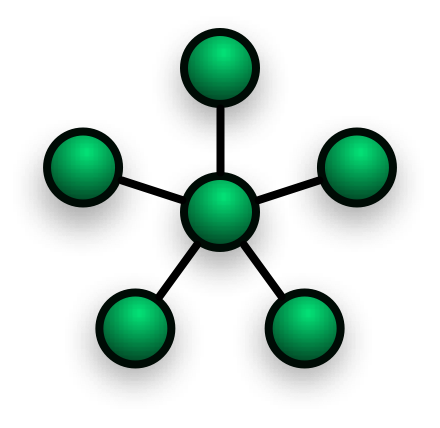
\includegraphics[width=0.5\textwidth]{NetworkTopology-Star.png}
\end{tabular}
\caption{
\label{fig:star} A star-topology 
\cite{lieberman2005evolutionary} . 
}
\end{figure}

The paper shows that in certain graphs this is possible, one example is the star topology \ref{fig:star}.
In this topology the fixation probability is\begin{equation}p_{2}=\frac{(1-1/r^{2})}{(1-1/r^{2N})} \label{eq:fixation2} \end{equation}.
or more generally: \begin{equation}
p_{k}=\frac{(1-1/r^{k})}{(1-1/r^{kN})} \label{eq:fixationk}
\end{equation}
And as we see when comparing \ref{eq:fixation} and \ref{eq:fixation2} the selective difference is
 amplified from $r$ to $r^{2}$, i.e. a star act as an evolutionary amplifier, favoring advantageous
  mutants and inhibiting disadvantageous mutants.
  
\subparagraph{endogenous and exogenous}
When analyzing networks it is important to differentiate between endogenous and exogenous network structures, it is easier to analyze exogenous networks, where the structure is given from the beginning. But networks where the structure is created by endogenous decisions are more natural and real world applicable. 

\subparagraph{An exogenous insurable topology}
When applying the results from \cite{lieberman2005evolutionary} to our scenario, cyber insurance and insurable topologies, we can use this to show
 that when given a star network structure, if the center node is strongly secured, then the virus will be considered as disadvantageous and
it will be inhibited from fixation with a certain probability. 
This makes the overall risk easier to calculate for both the insurer and the nodes,
and makes it possible and easier to calculate fair and affordable premiums. 
It can also be used as an incentive for the center node to buy insurance or security software, 
because it can easily be shown how probable an infection will occur. 

One could for example force the center node to buy sufficient anti virus, 
by informing it about how likely it will be infected, and how expensive the cyber insurance will be if 
it do not invest sufficiently in self protection. This will make the whole network more secure, 
and the insurer can now offer insurance to the leaf nodes for a fair price with a calculable risk. 
This could also be used to show how information about cyber-insurance or protection software will
spread throughout a network, and if the information is advantageous, eventually all nodes will acquire
the insurance or software.
    
There are other graphs where the fixation probability is equal to \ref{eq:fixationk}, funnel and
metafunnel. And as we know from chapter \ref{chp:graphTheory}, about graph theory, there are many
topologies in our society that are similar to these graphs.  In all of these, it can be
shown that if N is large enough, the fixation probability for advantageous mutant converges to 1, 
and for disadvantageous converges to 0.

\subsection{Network games}
In the paper \cite{networkgames} they show how network games evolve when the payoffs are determined not only by your own decisions, but also by your neighbours. 
A game that is applicable to our scenario is when considering security software, 
security software can be considered as a public good, it suffers from strategic substitutes, i.e. 
that if your neighbour acquire it, it gives you less incentive to also acquiring the software. 
Public goods and security also benefits from positive externalities, when one acquires the software, 
all the neighbours benefits from it, because the risk of being infected decreases.
Lets consider a simple game shown in this paper.
We have an action space: $X=\{0,1\}$, where 1 can be considered as acquiring information, take vaccine, buy security software etc. And 0 is not doing so.
Each node $i$ has a set of neighbours: $N_{i} $ and a payoff function $y_{i}=x_{i}+\bar{x}N_{i}$
The gross payoff of the game is 1 if $y_{i}>=1$ and 0 otherwise. There is a cost of choosing the action 1, and the cost is: $0<c<1$.
%% [location]h-here, t top, b bottom.
\begin{figure}[h]
\centering
\begin{subfigure}{.4\textwidth}
  \centering
  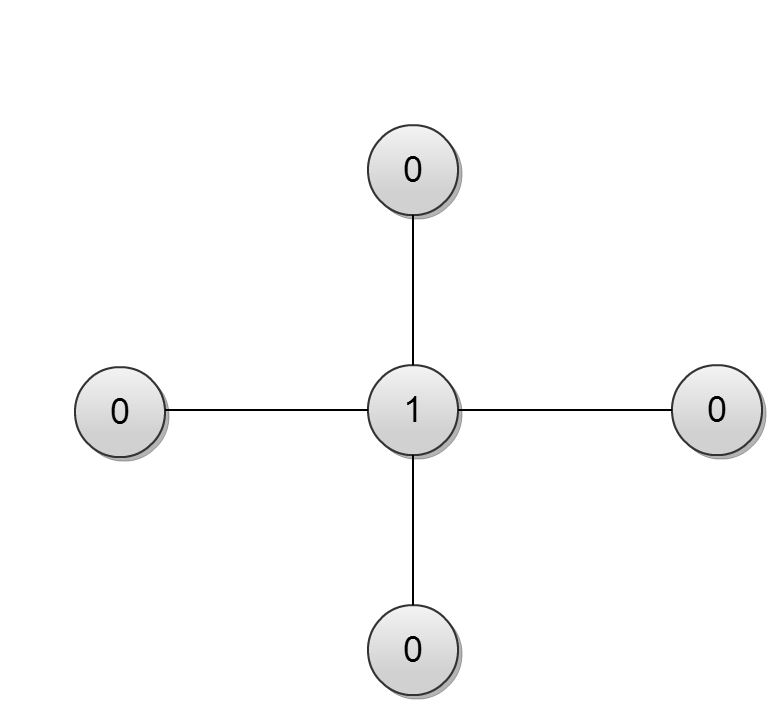
\includegraphics[width=0.8\linewidth]{optimalequilibrium.png}
  \caption{\label{fig:optequi} Socially Optimal equilibrium, center node choose action 1}
\end{subfigure}
\quad
\begin{subfigure}{.4\textwidth}
  \centering
  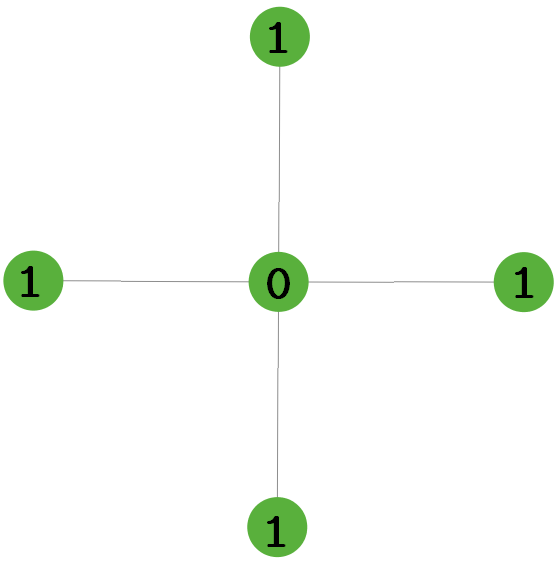
\includegraphics[width=0.8\linewidth]{notoptimalequilibrium.png}
  \caption{\label{fig:notoptequi} Non Socially Optimal equilibrium, leaf nodes choose action 1}
\end{subfigure}
\caption{\label{fig:starequi} Figure \ref{fig:optequi} shows the socially optimal equilibrium, and \ref{fig:notoptequi} shows the non optimal equilibrium.}

\end{figure}

 When we look at the star example, we easily see that there is two equilibriums \ref{fig:starequi}, one where the center node choose action 1 and the rest of the nodes choose action 0, and a second equilibrium where all the leaf nodes chooses 1 and the center choose 0.
The overall payoff in these two differ from each other, the latter is not socially optimal because it
 suffers from a cost equal to: $\#leaf nodes*c$ versus the first equilibrium where the total cost is only $c$.
If we could have forced the network game to end up in the socially optimal equilibrium, this would have been optimal. 
One possibility could be for the insurer to offer cheap insurance to all the leaf nodes, and a expensive one to the center node. By expensive we mean a cost that exceeds the cost of acquiring self protection, because then a rational center node would strictly prefer buying security software, as long as the price for acquiring and maintaining it is less than the possible cost of loss.
\begin{equation}
 U_{center}=-Probability_{casualty}*\alpha-Cost_{selfprotection}
 \label{eq:utility}
 \end{equation} 
A risk averse player would like to maximize her expected utility \ref{eq:utility}. We assume that the probability of casualty is significantly smaller when acquiring self protection, versus not acquiring. If the options for a player is
 either to remove the expected loss of casualty by acquiring self protection, or by insuring against it,
and the expected utility of acquiring insurance is lower than the expected utility of acquiring self protection. The player would strictly prefer self protection. 
This is a simple scenario, where the network formation is given in advance, exogenous network formation, 
but it shows how a insurer can force the game to end up in the social optimal equilibrium, by using the information about how fixation probability, and informing the players. 
And in this way creating a simple but insurable network topology. 

\section{Notater og slikt}

\section{NOTES... random.. don't read}

Thoughts on what this fixes in a simple way...
The insurer can now calculate the probability for catastrophic event(all nodes suffer), and now atleast has a measurement on the correlated risk. It has also limited the information asymmetry to concern only one node, the center node. It does not matter if the leaf nodes acquire security or not. Also it has now limited the interdependent security to one node, the center node.

 
The game:
The way this game works, is that we look at nodes that are mutated (A), and those who are not (B).  


When we apply the game to a directed graph, there are four different outcomes, a,b,c and d, which represents the interaction between the nodes, as is depicted in the figure below\ref{fig:game}. 

In the first figure (Positive symmetric) the fixation probability is related to r=b/c. If b is greater than c, the properties of mutant b will propagate in to all the other nodes, and the whole graph will eventually consists of only mutated nodes. The opposite will happen in the case where c is greater than b, leading to extinction of the mutation. The later scenario models the situation where proper protection against a mutant i.e. a security threat is installed. If the level of security, c is higher that the strength of the security threat it will be blocked from propagating further into the network. 


\begin{figure}[h]
\centering
\begin{tabular}{@{}c@{}}
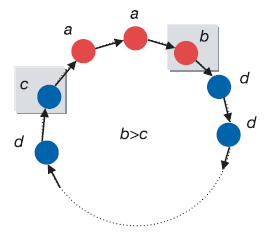
\includegraphics[width=0.5\textwidth]{natureGameSingle.png}
\end{tabular}
\caption{\label{fig:game} Mutant propagation game}
\end{figure}


More generalized, $W$ does not need to be stochastic, $w_{ij}>=0$. 
If the sum of all edges leaving a vertex is equal for all vertexes, then the graph will never suppress selection.
If the sum of all edges entering a vertex is equal for all vertexes, the graph never suppress drift.
If both then the graph is called a circulation.
     
To be able to point out insurable topologies, an extensive study of different graphs and how they behave has to be conducted. Regarding security, knowledge of how viruses spread and how to use graph structures to prevent malicious hackers from entering your network is important. Evolutionary dynamics, and the research of how mutant genes spread though out a population fits in to the model of security. 

Where the fixation probability determines the rate of evolution, which relies both on the size of the network and the evolution speed. A probability of 1 means that every node in the network eventually will be affected by the mutant.   
Isotherm graphs are a sub-graph of circulation. 

If $W$ is symmetric, or isotherm then the fixation probability is always \ref{eq:fixation}
isotherm means doubly stochastic, all rows and cols sum to 1. 
If a graph is one rooted, it has a fixation prob of $1/N$ regardless of $r$. If a graph has more then one root, its fixation probability is zero. 
Is it possible to find graphs with fixation probability that exceeds \ref{eq:fixation}? Is it possible to suppress drift and amplify selection?

And the selective difference is as we see amplified from $r$ to . i.e. a star act as an evolutionary amplifier,
 favoring advantageous mutants and inhibiting disadvantageous mutants, tilts towards selection and against drift.
 
 
 in certain graphs, star, funnel, metafunnel, if N is large enough, fixation probability for advantageous mutant converges to 1. Fixprob for disadvantageous converges to 0.
 
 
The same theory can be used to demonstrate how the aggregated security of a network is higher if the central node of a star structure is secured. 
If we assume that implemented security is 100$\%$ efficient, no threats will propagate beyond that node i.e total security for the network is increased. 
Scale-free networks have most of their connectivity clustered in a few vertices, i.e. they are potent selection amplifiers.